\documentclass[border=10pt]{standalone}
\usepackage{tikz}
\usetikzlibrary{arrows.meta, fit, calc, backgrounds, positioning}

% ── Colour palette ────────────────────────────────────────────────────────────
\definecolor{cQ} {RGB}{ 44,100,180}   % query  — deep blue
\definecolor{cR} {RGB}{ 32,138, 78}   % retrieval — forest green
\definecolor{cDB}{RGB}{115, 80,175}   % database  — purple
\definecolor{cC} {RGB}{205,105, 25}   % context   — amber
\definecolor{cL} {RGB}{165,115, 15}   % LLM       — golden
\definecolor{cN} {RGB}{130, 50,168}   % NLI       — violet
\definecolor{cO} {RGB}{ 22,128,110}   % output    — teal
\definecolor{cBd}{RGB}{172, 22, 22}   % boundary  — crimson

\tikzset{
  proc/.style={
    rectangle, rounded corners=4pt,
    draw=#1!80!black, fill=#1!14, text=#1!35!black,
    minimum width=24mm, minimum height=13mm,
    align=center, font=\small\bfseries,
    inner sep=4pt, line width=0.9pt
  },
  llmbox/.style={
    rectangle, rounded corners=4pt,
    draw=cL!80!black, fill=cL!14, text=cL!35!black,
    minimum width=28mm, minimum height=16mm,
    align=center, font=\small\bfseries,
    inner sep=5pt, line width=0.9pt
  },
  dbbox/.style={
    rectangle, rounded corners=3pt,
    draw=cDB!80!black, fill=cDB!14, text=cDB!35!black,
    minimum width=24mm, minimum height=13mm,
    align=center, font=\small\bfseries,
    inner sep=4pt, line width=0.9pt,
    double, double distance=1.6pt
  },
  fa/.style={->, >=Stealth[round], line width=1.6pt, draw=black!72},
  da/.style={->, >=Stealth[round], line width=1.0pt,
             draw=black!38, dashed, dash pattern=on 4pt off 2.5pt},
  sn/.style={circle, draw=black!28, fill=white, line width=0.5pt,
             inner sep=0pt, minimum size=5.2mm,
             font=\tiny\bfseries\color{black!60}},
  an/.style={font=\tiny\itshape, text=black!48, align=center},
}

\begin{document}
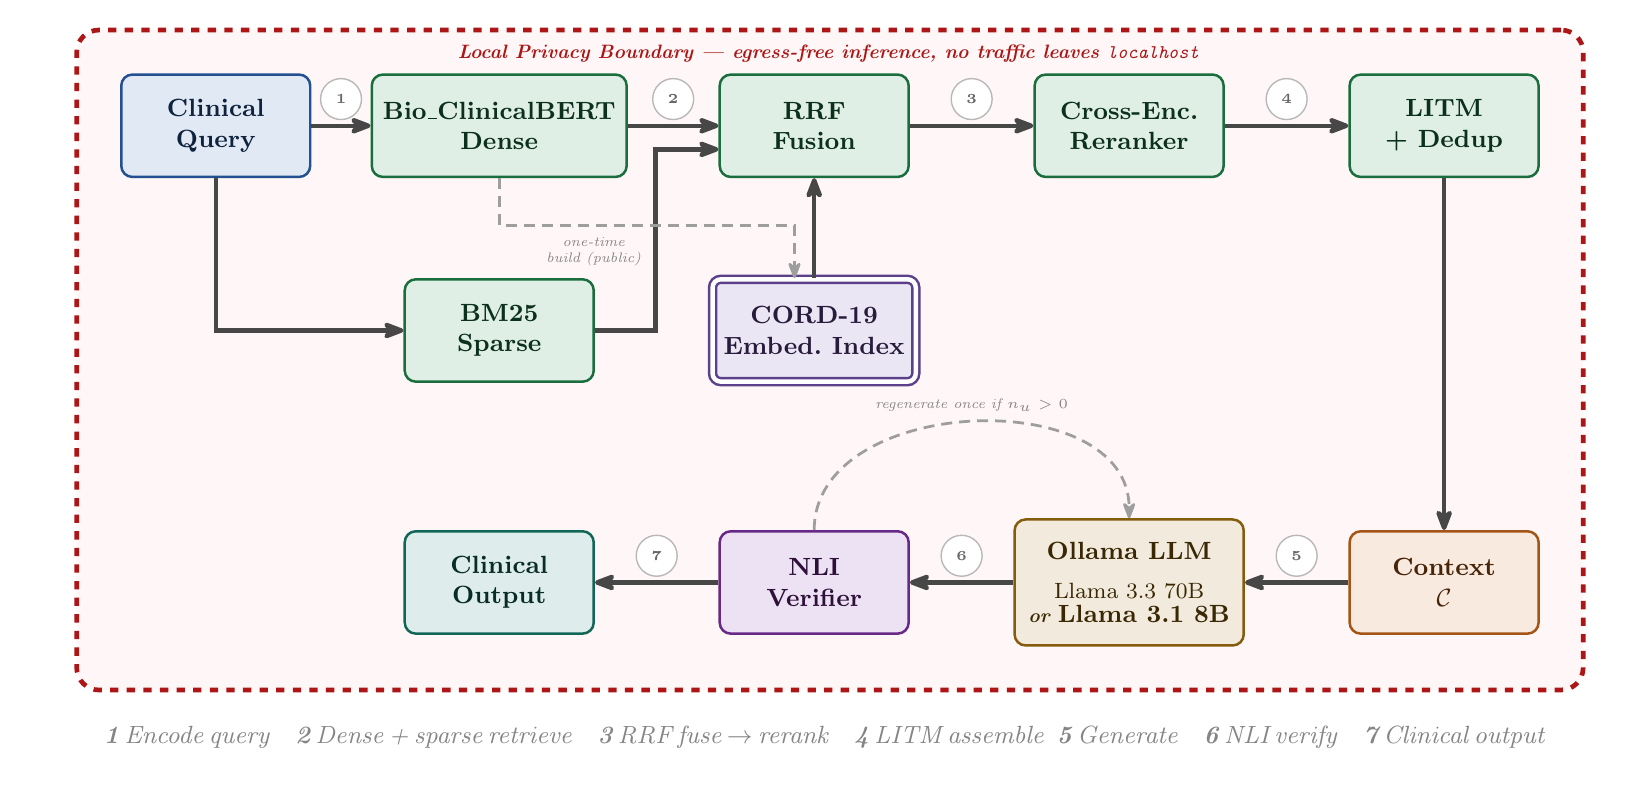
\begin{tikzpicture}

%% ── Top retrieval row (left → right, y = 0) ─────────────────────────────────
\node[proc=cQ] (query) at (  0mm,   0mm) {Clinical\\Query};
\node[proc=cR] (dense) at ( 36mm,   0mm) {Bio\_ClinicalBERT\\Dense};
\node[proc=cR] (rrf)   at ( 76mm,   0mm) {RRF\\Fusion};
\node[proc=cR] (ce)    at (116mm,   0mm) {Cross-Enc.\\Reranker};
\node[proc=cR] (litm)  at (156mm,   0mm) {LITM\\+ Dedup};

%% ── Middle row (y = –26 mm) ──────────────────────────────────────────────────
\node[proc=cR] (bm25) at ( 36mm, -26mm) {BM25\\Sparse};
\node[dbbox]   (db)   at ( 76mm, -26mm) {CORD-19\\Embed.\ Index};

%% ── Bottom generation row (right → left, y = –58 mm) ────────────────────────
\node[proc=cC]  (ctx) at (156mm, -58mm) {Context\\$\mathcal{C}$};
\node[llmbox]   (llm) at (116mm, -58mm)
  {Ollama LLM\\[3pt]\footnotesize\mdseries
   Llama 3.3 70B\\[-2pt]{\scriptsize\itshape or}\;Llama 3.1 8B};
\node[proc=cN]  (nli) at ( 76mm, -58mm) {NLI\\Verifier};
\node[proc=cO]  (out) at ( 36mm, -58mm) {Clinical\\Output};

%% ── Retrieval arrows ─────────────────────────────────────────────────────────
\draw[fa] (query.east)  -- node[sn, above=2pt]{1} (dense.west);
\draw[fa] (query.south) |- (bm25.west);

\draw[fa] (dense.east) -- node[sn, above=2pt]{2} (rrf.west);
\draw[fa] (bm25.east) -| ([yshift=-3mm,xshift=-8mm]rrf.west) -- ([yshift=-3mm]rrf.west);
\draw[fa] (db.north)   -- (rrf.south);

\draw[fa] (rrf.east) -- node[sn, above=2pt]{3} (ce.west);
\draw[fa] (ce.east)  -- node[sn, above=2pt]{4} (litm.west);
\draw[fa] (litm.south) -- (ctx.north);

%% ── Generation arrows ────────────────────────────────────────────────────────
\draw[fa] (ctx.west)  -- node[sn, above=2pt]{5} (llm.east);
\draw[fa] (llm.west)  -- node[sn, above=2pt]{6} (nli.east);
\draw[fa] (nli.west)  -- node[sn, above=2pt]{7} (out.east);

%% ── Offline indexing (dashed) ────────────────────────────────────────────────
\draw[da] (dense.south) -- ++(0,-6mm) -| ([xshift=-2.5mm]db.north);
\node[an] at (48mm, -16mm) {one-time\\build (public)};

%% ── Regeneration loop (dashed) ───────────────────────────────────────────────
\draw[da] (nli.north)
    to[out=90, in=90, looseness=1.1]
    node[an, above=0.1mm] {regenerate once if $n_u > 0$}
    (llm.north);

%% ── Privacy boundary ─────────────────────────────────────────────────────────
\begin{scope}[on background layer]
\node[
  draw=cBd, dashed, line width=1.7pt,
  fill=red!3, rounded corners=8pt, inner sep=5.5mm,
  fit=(query)(dense)(bm25)(rrf)(db)(ce)(litm)(ctx)(llm)(nli)(out),
  label={[font=\scriptsize\bfseries\color{cBd},
          anchor=north, inner sep=6pt]
         north:\textit{Local Privacy Boundary ---
                        egress-free inference, no traffic leaves \texttt{localhost}}}
] (bnd) {};
\end{scope}

%% ── Legend ───────────────────────────────────────────────────────────────────
\node[an,xshift=-7mm, anchor=north west, text width=200mm]
    at ($(bnd.south west)+(1mm,-3mm)$) {
    \small
  \textbf{1}~Encode query\enspace\enspace
  \textbf{2}~Dense + sparse retrieve\enspace\enspace
  \textbf{3}~RRF fuse $\to$ rerank\enspace\enspace
  \textbf{4}~LITM assemble\enspace
  \textbf{5}~Generate\enspace\enspace
  \textbf{6}~NLI verify\enspace\enspace
  \textbf{7}~Clinical output
};

\end{tikzpicture}
\end{document}
